\documentclass[11pt]{article}

\usepackage[margin=1in]{geometry}
\usepackage{setspace}
\usepackage{enumitem}
\usepackage{hyperref}
\usepackage[numbers]{natbib}
\usepackage{amsmath}
\usepackage{amssymb}
\usepackage{multirow}
\usepackage{booktabs}
\usepackage{float}
\usepackage{graphicx}
\usepackage{subcaption}

\setstretch{1.15}

\title{Fairness-Constrained Adversarial Training on Tabular Data}
\author{Jeremy Frank}
\date{\today}

\begin{document}
\maketitle

\begin{abstract}
% SKELETON NOTES:
% Four sentences, one per act plus result.
% 1. Adversarial attacks degrade tabular classifiers.
% 2. Madry-style training restores robustness but concentrates the gain in the
%    majority group, widening EOpp.
% 3. We embed a DPD constraint into the adversarial objective via augmented
%    Lagrangian.
% 4. Headline numbers: DPD reduction, robustness retained, and the overshoot /
%    sign-inversion finding from the tau sweep.
% Write this LAST.
\end{abstract}

\section{Introduction}\label{sec:introduction}
% SKELETON NOTES:
% - Motivate tabular fairness setting: Adult Income, consequential decisions,
%   protected attribute is sex.
% - State the gap: adversarial robustness literature is image-centric (Goodfellow,
%   Madry both MNIST/CIFAR); fairness literature (Hardt) is post-processing and
%   attack-agnostic. Little work sits at the intersection on tabular data.
% - State the three-act contribution explicitly as a bulleted list:
%     (1) characterize baseline vulnerability under FGSM/PGD in z-score epsilon units
%     (2) show Madry-style training trades EOpp for robustness, and diagnose why
%     (3) propose DPD-constrained adversarial training; report tau sweep frontier
%         and the EOpp sign-inversion result
% - One paragraph on paper organization.
% NO FIGURE HERE.

The last several years have brought about 


\section{Related Work}\label{sec:relatedwork}
% SKELETON NOTES: three short subsections, ~1 paragraph each. Pull from your
% existing summaries; cite, do not re-explain.

\subsection{Adversarial Examples and Robust Training}

Goodfellow et al.\ \cite{goodfellow2015} argue that adversarial examples arise not
from the non-linearity of deep networks, but from the combination of linear
structure and high input dimensionality. For a weight vector $w \in \mathbb{R}^n$
and a perturbation $\eta$ constrained by $\|\eta\|_\infty < \varepsilon$, the
perturbation changes the activation by $w^\top \eta$, which is maximized at
$\varepsilon m n$ where $m$ is the average magnitude of an element of $w$. The
damage therefore scales with the number of dimensions the attacker can move. From
this explanation the authors derive the Fast Gradient Sign Method, a single-step
attack that linearizes the loss and steps $\varepsilon$ in the direction of its
sign, and they propose training on FGSM examples as a form of regularization.

This premise does not transfer cleanly to our setting. We perturb only the six
continuous features of Adult, roughly $6\%$ of the feature space after one-hot
encoding, against the $784$ perturbable dimensions of an MNIST image. With $n$ this
small, the $\varepsilon m n$ argument predicts that conventional $\varepsilon$
values will have little effect, which is what we observe. We take this as
justification for the larger $\varepsilon$ range described in Section~2.2.3, and we
report $\varepsilon$ in standard-deviation units rather than as a fraction of
feature range.

Madry et al.\ \cite{madry2018} recast robustness as an optimization problem rather
than a property to be patched after the fact. Given a set of allowed perturbations
$S$, they formulate training as the saddle point problem
$$\min_\theta \; \mathbb{E}_{(x,y) \sim \mathcal{D}} \left[ \max_{\delta \in S}
L(\theta, x + \delta, y) \right],$$
where the inner maximization constructs a high-loss adversary and the outer
minimization fits parameters against it. Their central empirical claim is that the
inner problem, though non-concave, has local maxima tightly clustered in value, so
an approximate solution is good enough in practice. Projected Gradient Descent,
which iterates the sign-gradient step and projects back into the $\varepsilon$-ball,
produces the strongest first-order adversaries they tested and therefore the most
robust models. They further report that robustness depends on model capacity, and
that adversarial training can cause insufficiently large models to fail outright.

We adopt the saddle point formulation directly as the Act~2 training objective, and
PGD as our primary attack. Both papers evaluate on image data with convolutional
architectures; we apply the methods to tabular data with a logistic regression
baseline and a small MLP, where the capacity argument bears on our results in a way
we return to in the Discussion.

\subsection{Fairness Metrics}

Hardt et al.\ \cite{hardt2016} survey group fairness criteria for binary
classification and introduce two that condition on the true label. They begin from
demographic parity \cite{hardt2016}, which requires
$\Pr\{\hat{Y}=1 \mid A=0\} = \Pr\{\hat{Y}=1 \mid A=1\}$, and raise two objections to
it: a classifier can satisfy it by accepting unqualified individuals from one group
to match acceptance rates, and where the protected attribute is genuinely correlated
with the target, the criterion excludes the ideal predictor and forces a loss in
utility. In place of demographic parity they propose equalized odds, which requires
$\hat{Y}$ and $A$ to be independent conditional on $Y$, and the relaxation they call
equal opportunity, which imposes that condition only on the advantaged outcome group
$Y=1$ and therefore equalizes true positive rates alone. Their framework assumes the
target labels are themselves meaningful; where labels are noisy or biased, the
metrics inherit that bias.

We use these definitions as evaluation metrics rather than as the basis for a
post-processing step. Our constraint targets demographic parity, despite the
objections above, for reasons of estimation rather than normative preference. The
demographic parity difference admits a differentiable surrogate that averages over
every example in a minibatch, and is stable at our batch size of $32$. The equal
opportunity difference conditions on the joint $(A=a, Y=1)$ cell, which for the
minority group is small enough that the surrogate is unreliable per batch and the
reported metric carries substantial seed-to-seed variance. We therefore constrain
DPD during training and report EOpp as a secondary metric with per-seed spread. This
choice is a limitation as much as a design decision, and we return to it in
Section~7.

\subsection{Robustness--Fairness Interaction}
% - Tsipras et al. 2019 (robustness--accuracy tradeoff), Xu et al. 2021
%   (robust training has disparate effect), TRADES (Zhang et al. 2019).
% - Position your work: prior work observes the disparity; you constrain against it
%   during training on tabular data.

\section{Setup}\label{sec:setup}
% SKELETON NOTES: consolidate everything defined once so no act re-explains it.

\subsection{Data and Models}
% - Adult Income, OpenML id=1590. Protected attribute sex. G0 = male (majority),
%   G1 = female (minority). Give n, class balance, group sizes.
% - Logistic regression and small MLP. Give MLP width/depth, optimizer, batch size 32.
% - Preprocessing: one-hot categoricals, StandardScaler on 6 continuous features.

The dataset used is the OpenML 'adult' dataset (id=1590). The target column was encoded as 0 if the individual made less than 50k a year, and 1 otherwise. The protected attribute is sex; it is also binary encoded, with 0 denoting male and 1 denoting female. 

% Include figure of total rows, percentages of group 0 vs. group 1, number of features before and after one-hot encoding, and number / ratio of people in the advantaged outcome group per group. 

The dataset consists of 6 continuous and 8 categorical columns. We chose to use sklearn's StandardScaler and OneHotEncoder on the continuous and categorical features respectively. This gave us an end feature count of 102. 

On clean data, we observed an accuracy ceiling of ~.77 for the logistic model ~.79 for the MLP. The ceiling was invariant during tests of hidden dimension, epochs, number of layers, and more, indicating that the ceiling is set by feature overlap and not limitations of the model itself. We subsequently chose to use a small MLP with one hidden layer of 64 neurons, since its resulting accuracy differed only marginally from the observed ceiling.

Training ran for 40 epochs, with early stopping occurring after 10 epochs without improvement on the validation set. Both models used ADAM with learning rate .0001 and a batch size of 32.

\subsection{Threat Model}
% - FGSM and PGD definitions (lift from BaselineRobustnessEval memo verbatim).
% - PGD: 10 steps, alpha = 2*eps/steps, perturbation restricted to the 6 continuous
%   features only.
% - CRITICAL SUBSECTION: epsilon in z-score units. Lift the StandardScaler-vs-MinMax
%   argument from the baseline memo. State eps in {0, 0.1, 0.2, 0.3} and justify why
%   conventional {0.01, 0.03, 0.05} was inert. Putting this here means you never
%   defend it again.

\subsubsection{Fast Gradient Sign Method (FGSM)}

This algorithm linearizes the cost gradient function $J$ by taking the sign of each element and applying a constant size $\varepsilon$. That is, for a set of model parameters $\theta$, an input $x$, and a target output $y$, the FGSM perturbation is a single step in the direction of steepest loss increase,
$$\delta = \varepsilon\,\operatorname{sign}\!\left(\nabla_x J(\theta, x, y)\right),$$
giving the perturbed input $x^{adv} = x + \delta$.

\subsubsection{Projected Gradient Descent (PGD)}

PGD applies the same sign-gradient principle iteratively, taking smaller steps of
size $\alpha$ and projecting back into the $\varepsilon$-ball around $x$ after each step:
$$x^{adv}_{t+1} = \Pi_{x,\varepsilon}\!\left(x^{adv}_t + \alpha\,\operatorname{sign}\!\left(\nabla_x J(\theta, x^{adv}_t, y)\right)\right),$$
where $\Pi_{x,\varepsilon}$ projects onto the perturbation set: an $\varepsilon$-radius
$\ell_\infty$ ball centered at the original input $x$, restricted to continuous features.

\subsubsection{Choosing $\varepsilon$}
It took some experimentation to find effective values for $\varepsilon$ which affected performance but did not create model collapse. We began using the conventional values $\varepsilon = \{0.01, 0.03, 0.05\}$ and found that these did not meaningfully affect the model predictions. We formed two theories for why this occurs: 
\begin{itemize}
    \item \textbf{Low continuous feature dimension} \:\: We have restricted our perturbations to continuous features, of which there are only 6. This makes up ~$6\%$ of our feature space after one-hot encoding, and is a far cry from the 784 perturbable dimensions of an MNIST image.
    \item \textbf{Use of StandardScaler instead of MinMax} \:\: Since Adult has continuous features with extreme outliers (e.g.\ \texttt{capital\_gain}), we standardize with StandardScaler rather than the conventional MinMaxScaler. This changes what $\varepsilon$ means. Under MinMaxScaler, every feature is squeezed into $[0,1]$, so an $\varepsilon$-sized $\ell_\infty$ perturbation is a fraction of each feature's full observed range. Under StandardScaler, features are expressed in z-score units (mean $0$, standard deviation $1$), so $\varepsilon$ is measured in standard deviations: an $\varepsilon = 0.1$ perturbation moves a feature by one-tenth of a standard deviation, regardless of its raw range. A perturbation that is meaningful in $[0,1]$ units is therefore much larger in standard-deviation units, which is why the conventional $\varepsilon \in \{0.01, 0.03, 0.05\}$ had little effect and a larger $\varepsilon$ was needed to produce graded degradation. 
\end{itemize}
With these two considerations in mind, we swept larger $\varepsilon$ values, and found that meaningful model performance reductions occured around $\varepsilon \in [0.1, 0.3]$. For PGD we performed 10 steps of size $\alpha=\frac{2\varepsilon}{10}$. 

\subsection{Metrics}
% - Balanced accuracy, AUC, adversarial TPR, attack success rate.
% - DPD and EOpp with SIGNED convention. State explicitly:
%   positive => G0 has the higher rate. Both metrics use the same ordering.
% - Note the soft/hard DPD gap (surrogate reads ~5x lower); state that tau lives in
%   surrogate units and all reported DPD is hard-threshold.
% - Averaging protocol: seeds 0/1/2
%   State whether you report spread and where (appendix).

Our main effectiveness metric is balanced accuracy, and we use auc as a secondary metric. 

Let $\hat{Y}$ denote model predictions, $Y$ the true labels, and $A \in \{0,1\}$ a binary sensitive attribute. For a group $a$, we define the Positive Prediction Rate (PPR) and True Positive Rate (TPR) as
$$\text{PPR}_a = \Pr\{\hat Y = 1 \mid A=a\}, \quad \text{TPR}_a = \Pr\{\hat Y=1 \mid A=a, Y=1\}.$$

Our primary fairness metric, \textbf{Demographic Parity Difference (DPD)}, follows the principle of demographic parity: it measures the gap in positive prediction rates between groups,
$$\text{DPD} = \text{PPR}_0 - \text{PPR}_1$$
\textbf{Equal Opportunity Difference (EOpp)} applies the same construction to the positive class,
$$\text{EOpp} = \text{TPR}_0  - \text{TPR}_1$$
Both metrics are signed: a positive value indicates that group $0$ receives the higher rate.

All reported quantities are estimated on the held-out test set, e.g. $\widehat{\text{PPR}}_a = \frac{1}{n_a} \sum_{i:A_i=a} \hat{y_i}$ for $\hat{y_i} \in \{0,1\}$. 

These hard-threshold metrics are non-differentiable and cannot serve directly as training objectives. We therefore construct a differentiable by squaring the difference in aggregate probabilities, rather than the hard rates. It is important to note that because of this, the fairness tolerance $\tau$ introduced in section ~\ref{sec:singletolerance} is in squared units, and so is naturally smaller than the reported hard-label DPD. 

\section{Act 1: Baseline Vulnerability}\label{sec:act1}
% SKELETON NOTES:
% - Report ERM baseline under FGSM and PGD across epsilon.
% - Key observation to write up: FGSM and PGD are near-identical. Your explanation
%   (linear loss surface for logistic; constrained feature space + small capacity
%   for MLP) goes here. This justifies using PGD alone for the rest of the paper --
%   say that transition sentence explicitly.

Both baseline models suffer balanced accuracy and auc reductions when tested on FGSM adversarial examples. When tested on PGD samples, the models performed almost exactly the same, except for the MLP model performing worse at $\varepsilon = 0.3$. 

\begin{figure}[H]
    \centering
    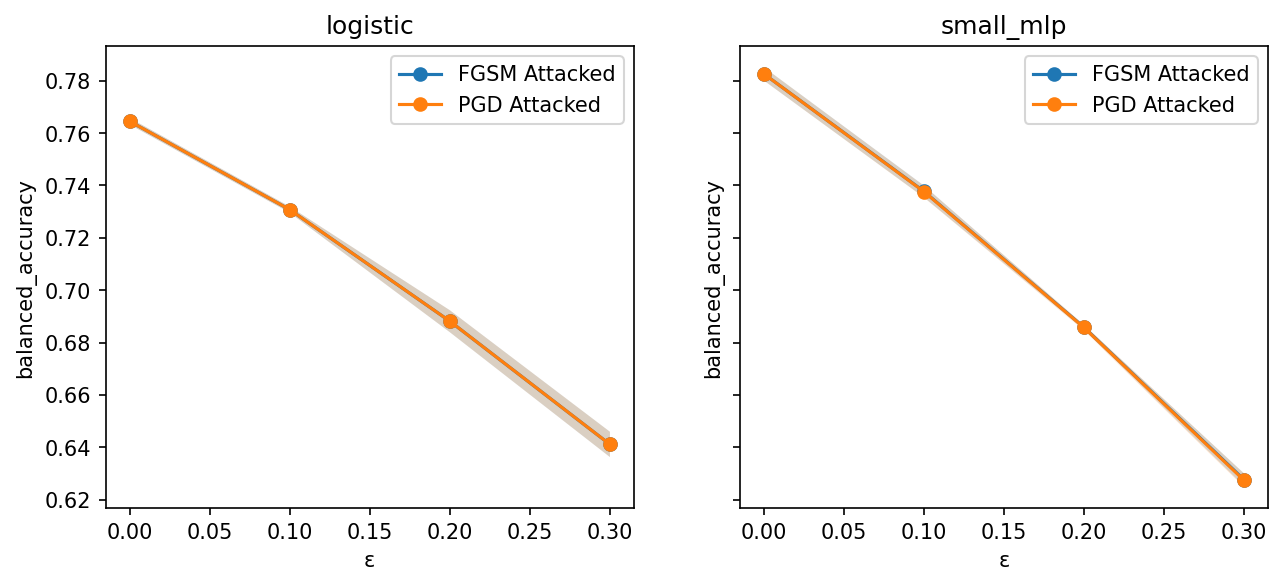
\includegraphics[width=0.75\linewidth]{../results/tables/fgsm_vs_pgd.png}
    \caption{Balanced accuracy vs. increasing epsilon values for both FGSM and PGD attacks}
    \label{fig:pgd_vs_fgsm}
\end{figure}

FGSM is expected to be near-optimal for the logistic model due to its linear loss surface and lack of an interior pathway for PGD to leverage. This would explain the identical effects of PGD and FGSM on the logistic model and also explain why the MLP suffers more from PGD. Since there is more non-linearity in MLP model it makes sense that it would perform worse under an attack designed to capture that nonlinearity. However, these improvements are limited due to constrained feature space and the small size of the model. 

Since PGD performs at least as well as FGSM for our models we decided to only focus on PGD moving forward. Full results tables are included in Appendix A. 

\begin{figure}[H]
    \centering
    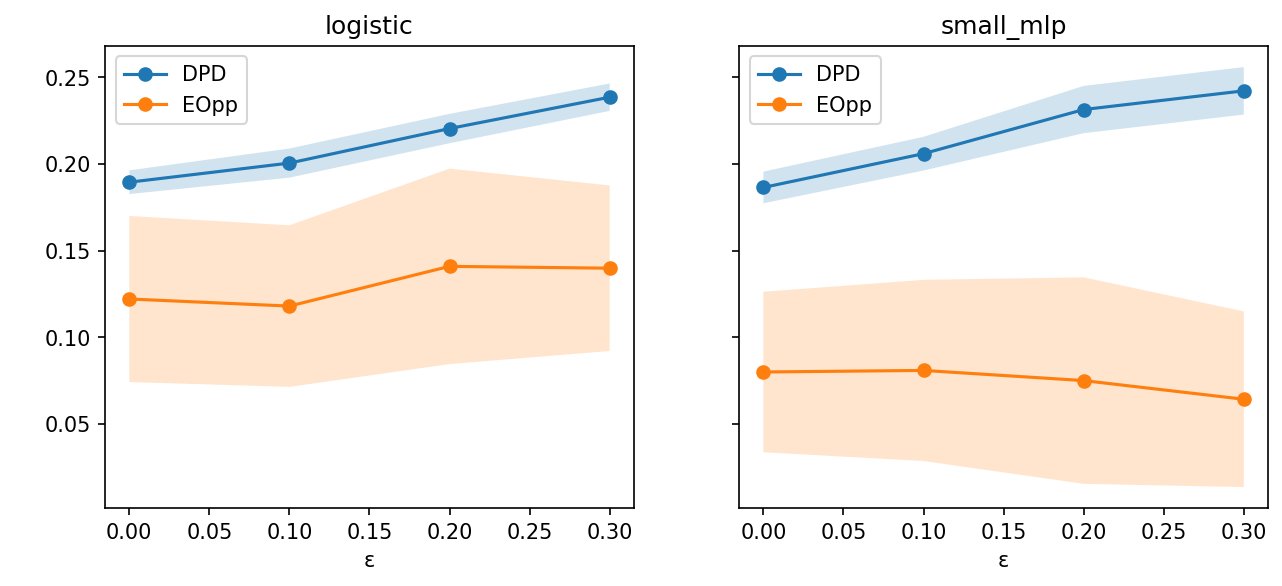
\includegraphics[width=0.75\linewidth]{../results/robustness/baseline/dp_eopp_baselines.png}
    \caption{Baseline DPD and Eopp Metrics with Standard Deviation and Increasing Epsilon}
    \label{fig:baseline_fairness}
\end{figure}
At baseline, we can see that DPD is increasing with high stability between runs, while EOpp remains stagnant with a high variance. Figure ~\ref{fig:act1_per_group} provide insight into how PGD attacks affect each model. 

\begin{figure}[H]
    \centering
    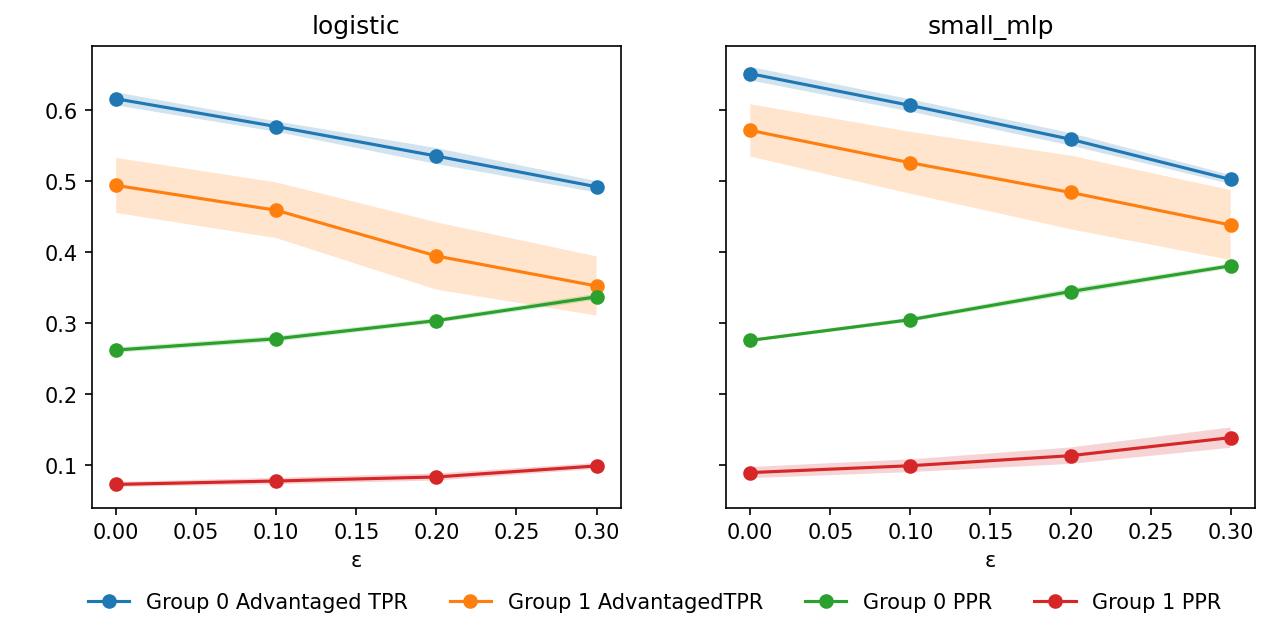
\includegraphics[width=0.75\linewidth]{../results/robustness/baseline/act1_per_group.png}
    \caption{Per-Group PPR and Advantaged TPR for Baseline Models}
    \label{fig:act1_per_group}
\end{figure}

Increasing positive prediction rates with falling advantaged true positive rates across all groups indicate that the attacks are successfully pushing negative samples into the positive prediction group. DPD widens because PPR's are increasing at a higher rate for the majority group, and EOpp is unstable because the minority group has a high standard deviation for advantaged TPR. This finding motivates our use of DPD as the primary fairness metric for this paper, though \cite{hardt2016} makes compelling arguments against it in favor of EOpp. Further research should be done averaging more seeds to examine the true behavior of EOpp under adversarial attacks. 

Given the behavior of our fairness metrics for the baseline model, it can be logically inferred that adversarial training will limit DPD increase under attack without mitigating the underlying fairness issues. 

\section{Act 2: Robust Training and Fairness Effects}\label{sec:act2}
% SKELETON NOTES:
% - Describe Madry-style adaptive training (min-max, per-batch PGD generation).
% - Static training in appendix
Our adversarial model employs an adaptive method of training in line with the saddle problem posed in \cite(madry2018). After a batch is selected, each sample in the batch is perturbed using the current model weights, and loss is calculated on the perturbed examples. This means the adversarial inputs being used for training can adapt to weight updates throughout training, creating a more robust model. Our unsuccessful static adversarial training run is included in the appendix. 

% - Balanced accuracy vs. baseline 
Adversarial training resulted in marked increases in balanced accuracy when tested againt perturbed inputs. This correlates with a decrease in attack success rate for all $\varepsilon$. There was also an expected marginal drop in accuracy on clean data.

\begin{figure}[H]
    \centering
    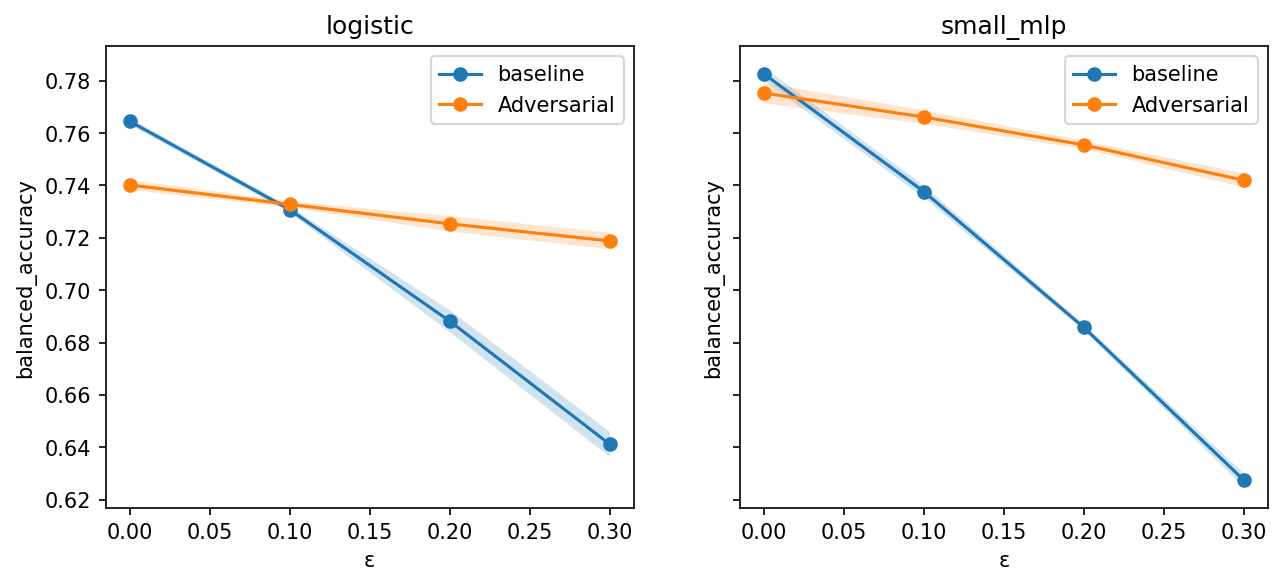
\includegraphics[width=0.75\linewidth]{../results/tables/act2acc.png}
    \caption{Accuracy}
    \label{fig:act2_accuracy}
\end{figure} 

% - DP & EOpp vs baseline
The behavior of the fairness metrics follows the hypothesis made at the end of Act \ref{sec:act1}. Table \ref{fig:act2_dp} 

% - Per-group PPR vs baseline. 



\section{Act 3: DPD-Constrained Adversarial Training}

\subsection{Formulation}
% SKELETON NOTES: lift from the July 24 memo with THREE CORRECTIONS:
%   (i) verify Lagrangian term signs match code (should be +)
%   (ii) lambda update must accumulate: lambda_{k+1} = max(0, lambda_k + eta*G_k)
%   (iii) mu schedule feasibility guard -- check the case conditions; the second
%         condition currently reads G_{k-1} > 0 and should likely be G_k > 0
% - G(theta) = |DPD_soft(theta)| - tau. State the absolute value explicitly;
%   without it the constraint is one-sided.
% - Note KKT dual feasibility as the reason lambda is floored at 0.
% - Cite Nocedal & Wright for the augmented Lagrangian / penalty schedule.

\subsection{Implementation Notes}
% SKELETON NOTES: short subsection, but a reviewer will want each of these.
% - Soft sigmoid DPD surrogate; verified ~0.030 soft vs ~0.17 hard on the Madry
%   model. Hence tau = 0.015 is not as small as it looks.
% - Empty-group minibatches return nan by design; guarded at batch loss and lambda
%   update rather than silently suppressed.
% - Feasibility-first early stopping: best val loss among constraint-satisfying
%   epochs. Requiring fairness to improve monotonically kills training, since DPD
%   naturally rises as the model learns.
% - Raised patience so training survives the constrained adaptation phase
%   (visible accuracy dip while the constraint binds).
% - PGD attack cache keyed on tau.
% - Initialization lambda=0, mu=1; untrained model is trivially fair.
% - Optional: note mu saturates at its doubling ceiling but is inert while the
%   constraint is slack, so it does not affect the converged solution.

\subsection{Results at \texorpdfstring{$\tau = 0.015$}{tau = 0.015}}\label{sec:singletolerance}
% SKELETON NOTES:
% - Report Fair vs Madry. DPD drops substantially; robustness retained
%   (attack success comparable or better).
% - THE HONEST PART: EOpp does not merely shrink, it overshoots. Per-group numbers
%   show G1 adversarial TPR up ~21 points while G0 drops ~3 (logistic).
%   Frame this as: DP-constrained training equalizes positive RATES, which
%   overcorrects TPR. This is an argument that DPD is the wrong constraint target
%   for EOpp, not a failure of the method.
% - Forward-reference the tau sweep as evidence.

\begin{figure}[H]
% FIGURE 4: Per-group effect of the constraint.
% Grouped bars: delta adversarial TPR (Fair - Madry), G0 vs G1, both architectures,
% at eps = 0.3.
% Purpose: makes the overshoot visible and unmissable. Do not hide this.
\caption{The DPD constraint redistributes true positive rate between groups.}
\label{fig:act3_pergroup}
\end{figure}

\subsection{Constraint Strength Sweep}
% SKELETON NOTES:
% - tau in {0.005, 0.01, 0.015, 0.02, 0.025}, both architectures, 3 seeds.
% - Finding 1: DPD and balanced accuracy trade off monotonically and smoothly.
%   Tightening tau buys fairness, costs accuracy.
% - Finding 2 (the interesting one): EOpp is non-monotonic in tau under the
%   absolute-value metric, bottoming near tau = 0.02. With SIGNED EOpp, interpret
%   as: tight tau overshoots into reverse disparity (G1 above G0), loose tau
%   retains original disparity, and the path CROSSES THROUGH equality.
%   DP-constrained training passes through EOpp-optimality rather than
%   approaching it.
% - Only write Finding 2 after the signed recomputation confirms the crossing.

\begin{figure}[H]
% FIGURE 5: Fairness--accuracy frontier.
% Scatter: x = DPD, y = balanced accuracy. One point per tau, labeled.
% Two series (logistic, MLP) or two panels. Include the unconstrained Madry point
% as an anchor so the reader sees where the frontier starts.
% Purpose: the standard fairness-paper framing. "You pay this much accuracy for
% this much fairness."
\caption{Fairness--accuracy tradeoff frontier across constraint strengths.}
\label{fig:act3_frontier}
\end{figure}

\begin{figure}[H]
% FIGURE 6: The sign inversion. SEPARATE FIGURE -- do not merge into Figure 5.
% x = tau; y = SIGNED EOpp. Horizontal rule at y = 0.
% Two lines (logistic, MLP). Mark the zero crossing.
% Purpose: this is your most novel finding. A monotonic panel would bury it.
\caption{Signed equal opportunity difference crosses zero as the constraint relaxes.}
\label{fig:act3_signflip}
\end{figure}

\section{Discussion}
% SKELETON NOTES:
% - Synthesize the arc: robustness is not group-neutral; constraining the wrong
%   fairness metric overcorrects; the constraint strength is itself a fairness
%   parameter with a non-monotonic effect on the metric you may actually care about.
% - Practical implication: if EOpp is the target, DPD-constrained training can hit
%   it, but only at a specific tau found by sweeping -- it is not the limit as
%   tau -> 0. That is a genuinely useful, slightly surprising claim.
% - Architecture comparison: the effect is much stronger in logistic than MLP.
%   Say why you think so (capacity, decision boundary flexibility) or say you
%   do not know.

\section{Limitations and Future Work}\label{sec:limitations}
% SKELETON NOTES:
% - EOpp-constrained training deferred: joint (group, positive-label) cell too
%   small at batch size 32. This is the obvious next experiment; name it.
% - Only 6 perturbable dimensions; epsilon in z-score units is a reporting
%   convention, not a normed-input-space guarantee. Results may not transfer to
%   MinMax-scaled setups.
% - Three seeds only.
% - Single dataset, single protected attribute, binary groups.
% - Static PGD augmentation was attempted and failed due to label leaking
%   (mention briefly here or in an appendix; it is a real negative result but
%   it is not part of the three-act story).

\appendix
\section{Full Result Tables}
% SKELETON NOTES:
% - Raw metric tables for all four regimes: ERM baseline, Madry, Fair (tau=0.015),
%   full tau sweep. Per-group breakdowns.
% - Each caption must be SELF-SUFFICIENT: seeds averaged, scores = value*100,
%   epsilon in z-score units, G0 = male/majority and G1 = female/minority,
%   sign convention for DPD and EOpp.
% - Report spread (std or min/max over seeds) here even if the main-text figures
%   use bands.

\begin{table}[H]
\centering
\caption{3-seed averages of FGSM (left) and PGD (right) attack results over all classes. Values are near-identical, justifying the use of PGD alone in subsequent sections.}
\label{tab:fgsm_pgd}
\begin{minipage}{0.49\textwidth}
\centering
\begin{tabular}{llrrr}
\toprule
Model & $\varepsilon$ & Bal.\ Acc. & DPD & EOpp \\
\midrule
\multirow{4}{*}{Log.}
 & 0.00 & 0.7645 & 0.1895 & 0.1221 \\
 & 0.10 & 0.7308 & 0.2005 & 0.1180 \\
 & 0.20 & 0.6882 & 0.2204 & 0.1409 \\
 & 0.30 & 0.6412 & 0.2385 & 0.1398 \\
\midrule
\multirow{4}{*}{MLP}
 & 0.00 & 0.7827 & 0.1864 & 0.0799 \\
 & 0.10 & 0.7378 & 0.2059 & 0.0808 \\
 & 0.20 & 0.6859 & 0.2310 & 0.0748 \\
 & 0.30 & 0.6277 & 0.2414 & 0.0635 \\
\bottomrule
\end{tabular}
\subcaption{FGSM}
\end{minipage}
\hfill
\begin{minipage}{0.49\textwidth}
\centering
\begin{tabular}{llrrr}
\toprule
Model & $\varepsilon$ & Bal.\ Acc. & DPD & EOpp \\
\midrule
\multirow{4}{*}{Log.}
 & 0.00 & 0.7645 & 0.1895 & 0.1221 \\
 & 0.10 & 0.7308 & 0.2005 & 0.1180 \\
 & 0.20 & 0.6882 & 0.2204 & 0.1409 \\
 & 0.30 & 0.6412 & 0.2385 & 0.1398 \\
\midrule
\multirow{4}{*}{MLP}
 & 0.00 & 0.7827 & 0.1864 & 0.0799 \\
 & 0.10 & 0.7377 & 0.2059 & 0.0808 \\
 & 0.20 & 0.6858 & 0.2314 & 0.0750 \\
 & 0.30 & 0.6275 & 0.2422 & 0.0642 \\
\bottomrule
\end{tabular}
\subcaption{PGD}
\end{minipage}
\end{table}

\section{FGSM Results}
% SKELETON NOTES: FGSM tables, since the main text argues FGSM ~ PGD and then
% uses PGD throughout.

\section{Static PGD Augmentation (Negative Result)}
% SKELETON NOTES: brief writeup of the label-leaking failure. Include the
% diagnostic reasoning (accuracy exceeded the baseline ceiling, which is
% impossible if the baseline was capped by feature overlap, not training).

\bibliographystyle{plainnat}
\bibliography{references}

\end{document}
